\documentclass[10pt,aspectratio=43]{beamer}
\usetheme{CambridgeUS}
\usecolortheme{dolphin}
\usepackage{multimedia}
\usepackage{xcolor}
\usepackage{graphicx}
\usepackage[normalem]{ulem}
\usepackage{amsmath}
\usetikzlibrary{positioning, shapes.geometric, arrows.meta}
\usepackage{pgfplots}
\pgfplotsset{compat=1.17}
% Graphics path for MasterTheorem figures
\graphicspath{{figures/MasterTheorem/}}
\begin{document}

%--------------------------------------------------------------------------- SLIDE 1 recap----------------------------------------------------------------------------------------
\begin{frame}
  \frametitle{Recap}
  \begin{itemize}

    \item \textbf{Recursion:} A problem-solving technique where a function calls itself to solve smaller instances of the same problem.
    
    \vspace{5pt}
    \begin{itemize}
        \item \textbf{Tree Method}  
         	\begin{itemize}
		        \item Visualizes the recursive calls as a tree.
		        \vspace{3pt}
		        \item Helps in making an   \textbf{educated guess} for the time complexity by summing the work done at each level of the tree.
    	    \end{itemize}
        \vspace{5pt}



        \item \textbf{Substitution Method} 
        \vspace{3pt}
        	\begin{itemize}
		        \item Used to \textbf{verify} the correctness of a guessed solution.
		        \vspace{3pt}
		        \item Proving the guess using induction (base case and inductive step).
    	    \end{itemize}
	    
	    
	    
        \vspace{5pt}
        \item \textbf{Master Theorem} 
                	\begin{itemize}
       	\item  Provides a direct way to solve recurrence relations.
	    	    \end{itemize}
    \end{itemize}
  \end{itemize}
\end{frame}

%--------------------------------------------------------------------------- SLIDE 2  divide & conquer ----------------------------------------------------------------------------------------
\begin{frame}
  \frametitle{Divide \& Conquer Example: Median of Medians}
  
  \textbf{Problem:} Find the median of an unsorted array efficiently.
  
  \begin{itemize}
      \item \textbf{Divide:}
      \begin{itemize}
          \item Split the array into groups of 5 elements
          \item Find the median of each group
          \item Recurse on the list of medians to find the ``median of medians"
      \end{itemize}
      \vspace{0.2cm}
      \item \textbf{Conquer:}
      \begin{itemize}
          \item Use the pivot to partition the array into:
          \begin{itemize}
              \item Elements less than the pivot
              \item Elements greater than the pivot
          \end{itemize}
          \item Recurse on the appropriate subarray to find the median
      \end{itemize}
      \vspace{0.2cm}
      \item \textbf{Combine:} 
      \begin{itemize}
          \item The pivot itself is the median or is used in further recursion
      \end{itemize}
  \end{itemize}
\end{frame}
%--------------------------------------------------------------------------- SLIDE 3  Time complex of D&C for ----------------------------------------------------------------------------------------
\begin{frame}
  \frametitle{Time Complexity Analysis}

  \textbf{Time Complexity:}
  \begin{itemize}
      \item \textbf{Divide:} \(T(n/5)\) — recurse on the list of medians.
      \item \textbf{Conquer:} \(T(7n/10)\) — recurse on the larger subarray.
      \item \textbf{Combine:} \(O(n)\) — partition the array around the pivot.
      \item \textbf{Overall:} \(T(n) = T(n/5) + T(7n/10) + O(n) \Rightarrow O(n)\).
  \end{itemize}
\end{frame}

%--------------------------------------------------------------------------- SLIDE 4 Big O--------------------------------------------------------------------------------------

\begin{frame}
  \frametitle{Recap of Asymptotic Notation: Big O (Upper Bound)}

  \begin{block}{Definition:} $f(n) = O(g(n))$ if $\exists$ constants $c > 0$ and $n_0 \geq 1$ such that:
\[
f(n) = O(g(n)) \iff  f(n) \leq c \cdot g(n) \quad \forall n \geq n_0, \quad \exists c > 0, \, n_0 \geq 1
\]
        \end{block}
          \begin{columns}

    \begin{column}{0.7\textwidth}
      \begin{itemize}
        \item \textbf{Intuition:}
        \begin{itemize}
            \item \( f(n) \) grows \textbf{no faster} than \( g(n) \).
            \vspace{3pt}
            \item Describes the \textbf{upper bound} on growth.
        \end{itemize}
        
        \item \textbf{Example:}
        \begin{itemize}
            \item If \( f(n) = 3n^2 + 2n + 1 \), then \( f(n) = O(n^2) \).
            \vspace{3pt}
            \item Here, \( c = 4 \) and \( n_0 = 1 \) satisfy the definition.
        \end{itemize}
      \end{itemize}
    \end{column}

    \begin{column}{0.3\textwidth}
      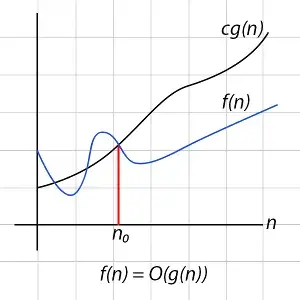
\includegraphics[width=\textwidth]{figures/MasterTheorem/big_o.jpg}
    \end{column}
  \end{columns}
\end{frame}

%--------------------------------------------------------------------------- SLIDE 5----------------------------------------------------------------------------------------
\begin{frame}
  \frametitle{Recap of Asymptotic Notation: Big Omega (Lower Bound)}

  \begin{block}{Definition:}
          \( f(n) = \Omega(g(n)) \) if $\exists$ constants $c > 0$ and $n_0 \geq 1$ such that:
          
\[
f(n) = \Omega(g(n)) \iff f(n) \geq c \cdot g(n) \quad \forall n \geq n_0,
 \quad \exists n_0 \geq 1, \quad 0 < c \leq 1
\]
\end{block}
  \begin{columns}
    \begin{column}{0.7\textwidth}
          \begin{itemize}
        \item \textbf{Intuition:}
        \begin{itemize}
            \item \( f(n) \) grows \textbf{no slower than} \( g(n) \).
            \vspace{3pt}
            \item Describes the \textbf{lower bound} on growth.
        \end{itemize}
        \item \textbf{Example:}
        \begin{itemize}
            \item If \( f(n) = 3n^2 + 2n + 1 \), then \( f(n) = \Omega(n^2) \).
            \vspace{3pt}
            \item Here, \( c = 3 \) and \( n_0 = 1 \) satisfy the definition.
        \end{itemize}
      \end{itemize}
    \end{column}

    \begin{column}{0.3\textwidth}
      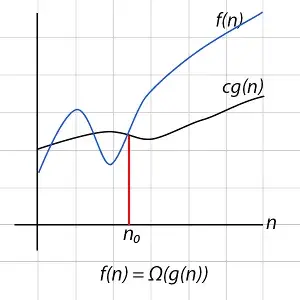
\includegraphics[width=\textwidth]{figures/MasterTheorem/omega.jpg}
    \end{column}
  \end{columns}
\end{frame}

%--------------------------------------------------------------------------- SLIDE 3 ----------------------------------------------------------------------------------------
\begin{frame}
  \frametitle{Recap of Asymptotic Notation: Big Theta (Tight Bound)}

  \begin{block}{Definition:}
          \( f(n) = \Theta(g(n)) \) if $\exists$ constants $c_1, c_2 > 0$ 
          \land $n_0 \geq 1$ such that:
\[
f(n) = \Theta(g(n)) \iff f(n) = O(g(n)) \text{ and } f(n) = \Omega(g(n))
\]
\end{block}
  \begin{columns}

    \begin{column}{0.7\textwidth}
      \begin{itemize}
        \item \textbf{Intuition:}
        \begin{itemize}
            \item \( f(n) \) is \textbf{asymptotically equal} to \( g(n) \).
            \vspace{3pt}
            \item \( f(n) = O(g(n)) \) and \( f(n) = \Omega(g(n)) \) simultaneously.
        \end{itemize}
        \item \textbf{Example:}
        \begin{itemize}
            \item If \( f(n) = 3n^2 + 2n + 1 \), then \( f(n) = \Theta(n^2) \).
            \vspace{3pt}
            \item Here, \( c_1 = 3 \), \( c_2 = 4 \), and \( n_0 = 1 \) satisfy the definition.
        \end{itemize}
      \end{itemize}
    \end{column}

    \begin{column}{0.3\textwidth}
      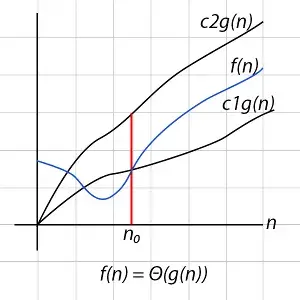
\includegraphics[width=\textwidth]{figures/MasterTheorem/theta.jpg}
    \end{column}
  \end{columns}
\end{frame}

%--------------------------------------------------------------------------- SLIDE 4 ----------------------------------------------------------------------------------------
\begin{frame}
  \frametitle{Little o}
 
  \begin{block}{Definition:}
        $f(n) = o(g(n))$ if for \textbf{every} constant $c > 0$, there exists a constant $n_0 \geq 1$ such that:
        \[
        0 \leq f(n) < c \cdot g(n) \quad \forall n \geq n_0
        \]
        \end{block}
         \begin{columns}
    % TEXT
    \begin{column}{0.7\textwidth}
      \begin{itemize}
        \item \textbf{Intuition}:  
        - $f(n)$ grows \textbf{strictly slower} than $g(n)$.  
        - Unlike Big O, this is a \textbf{non-tight} upper bound.  
        \vspace{5pt}
%        \item \textbf{Example}:  
%        - $f(n) = 2n + 3$ is $o(n^2)$ because $2n + 3$ grows slower than $n^2$ for large $n$.  
%        - However, $f(n) = 2n + 3$ is \textbf{not} $o(n)$ because $2n + 3$ grows at the same rate as $n$.
     \end{itemize}
    \end{column}

    % IMAGE
    \begin{column}{0.3\textwidth}
      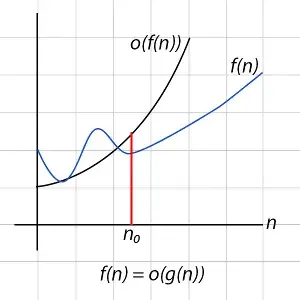
\includegraphics[width=\textwidth]{figures/MasterTheorem/little_o.jpg}
    \end{column}
  \end{columns}
\end{frame}

%--------------------------------------------------------------------------- SLIDE 8----------------------------------------------------------------------------------------------------
\begin{frame}
  \frametitle{Little $\omega$}

  \begin{block}{Definition:}
        $f(n) = \omega(g(n))$ if for \textbf{every} constant $c > 0$, there exists a constant $n_0 \geq 1$ such that:
        \[
          0 \leq c \cdot g(n) < f(n) \quad \forall n \geq n_0
        \]
\end{block}
        
  \begin{columns}

    \begin{column}{0.7\textwidth} 
      \begin{itemize}
        \item \textbf{Intuition}:  
        - $f(n)$ grows \textbf{strictly faster} than $g(n)$.  
        - Unlike Big Omega, this is a \textbf{non-tight} lower bound.  
        \vspace{3pt}
%        \item \textbf{Example}:  
%        - $f(n) = n^2$ is $\omega(n)$ because $n^2$ grows faster than $n$ for large $n$.  
%        - However, $f(n) = n^2$ is \textbf{not} $\omega(n^2)$ because they grow at the same rate.
      \end{itemize}
    \end{column}

    \begin{column}{0.3\textwidth} 
      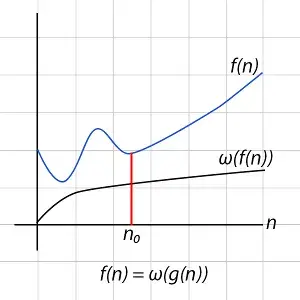
\includegraphics[width=\textwidth]{figures/MasterTheorem/little_omega.jpg}
    \end{column}
  \end{columns}
\end{frame}

%--------------------------------------------------------------------------- OPTIONAL ----------------------------------------------------------------------------------------------------

%\begin{frame}
%  \frametitle{Comparison of Little o and Little $\omega$}
%  \begin{itemize}
%    \item \textbf{Key Differences from Big O and Big Omega:}
%    
%    \vspace{5pt}
%    
%    \begin{itemize}
%      \item \textbf{Little o}:  
%      - Represents a \textbf{strictly smaller} growth rate than Big O.  
%      - Example: $n = o(n \log n)$, but $n \neq o(n)$.  
%      \item \textbf{Little $\omega$}:  
%      - Represents a \textbf{strictly larger} growth rate than Big Omega.  
%      - Example: $n^2 = \omega(n)$, but $n^2 \neq \omega(n^2)$.
%    \end{itemize}
%
%\end{frame}

\begin{frame}
  \frametitle{Master Theorem}
  The Master Theorem determines the asymptotic time complexity $T(n)$ by comparing $f(n)$ with $O(n^{\log_b a})$. The final complexity depends on which term dominates.
  \begin{center}
      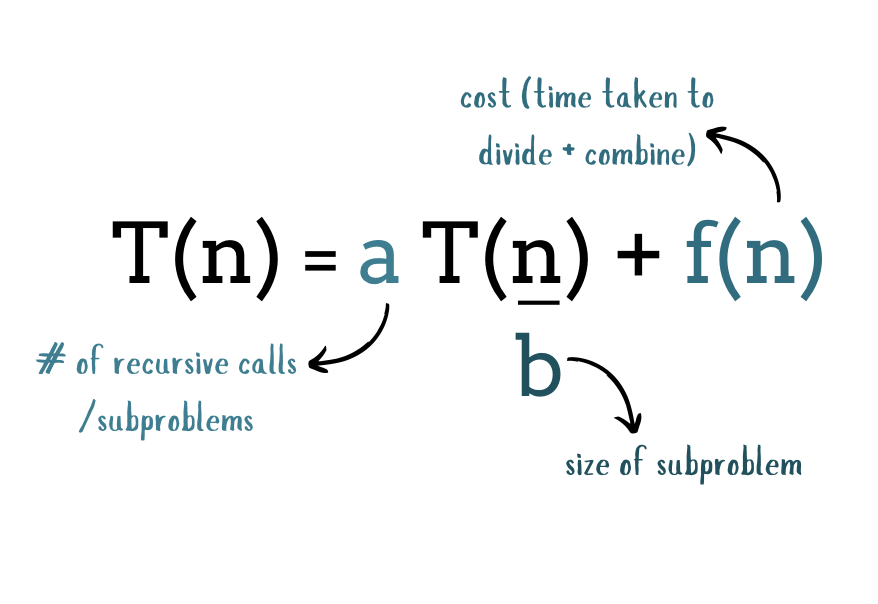
\includegraphics[width=0.6\textwidth]{figures/MasterTheorem/mt.jpg}
   \end{center}
  
\end{frame}


%--------------------------------------------------------------------------- SLIDE  MASTER THEOREM CASES----------------------------------------------------------------------------------------------------
%------CASE 1
\begin{frame}{Case 1: Cost remains equal to each level}

\begin{block}{}
\[
f(n) = \Theta(n^{\log_b a})
\]
\[
T(n) = f(n) \cdot \log n = \Theta(n^{\log_b a} \cdot \log n)
\]
\end{block}

\begin{itemize}
    \item \textbf{Intuition}:
    \begin{itemize}
            \item The cost \( f(n) \) is \textbf{equal} to \( n^{\log_b a} \) at every level.


    \end{itemize}
\end{itemize}

\end{frame}

%------CASE 2
\begin{frame}{Case 2: Cost decreases at each level}

\begin{block}{}
\[
f(n) = o(n^{\log_b a})
\]
\[
T(n) = \Theta(n^{\log_b a})
\]
\end{block}

\begin{itemize}
    \item \textbf{Intuition}:
    \begin{itemize}
        \item The cost \( f(n) \) is \textbf{asymptotically smaller} than \( n^{\log_b a} \).
    \end{itemize}
\end{itemize}

\end{frame}

%------CASE 3
\begin{frame}{Case 3: Cost increases at each level}

\begin{block}{}
\[
f(n) = \omega(n^{\log_b a})
\]
\[
T(n) = \Theta(f(n))
\]
\end{block}

\begin{itemize}
    \item \textbf{Intuition}:
    \begin{itemize}
        \item The cost \( f(n) \) is \textbf{asymptotically larger} than \( n^{\log_b a} \).

    \end{itemize}
\end{itemize}

\end{frame}
%----------- TERMONOLOGY DIFFERENCE
\begin{frame}{Book vs Professor's Terminology: Asymptotic Equivalences}

  \begin{block}{Case 2: Growth Rate Below Threshold}
    \[
    f(n) = o(n^{\log_b a}) \iff f(n) = O(n^{\log_b{a-\epsilon}}), \quad \epsilon > 0
    \]
  \end{block}

  \vspace{0.5cm}

  \begin{block}{Case 3: Growth Rate Above Threshold}
    \[
    f(n) = \omega(n^{\log_b a}) \iff f(n) = \Omega(n^{\log_b{a+\epsilon}}), \quad \epsilon > 0
    \]
  \end{block}

\end{frame}
%--------------------------------------------------------------------------- EXAMPLE 1----------------------------------------------------------------------------------------------------


\begin{frame}{Example 1}
  \begin{block}{Recurrence}
\[
T(n) = 8T(n/2) + cn
\]
  \end{block}

\textbf{Solution:}
\begin{itemize}
    \item Compare \( f(n) = cn \) with \( n^{\log_b a} = n^{\log_2 8} = n^3 \).
    \item Since \( f(n) = O(n^{\log_b a - \epsilon}) \) for \( \epsilon > 0 \), \textbf{Case 2} applies.
    \item \( T(n) = \Theta(n^3) \).
\end{itemize}
\end{frame}

%--------------------------------------------------------------------------- EXAMPLE 2---------------------------------------------------------------------------------------------------

\begin{frame}{Example 2}
\frametitle{Example 2}
  \begin{block}{Recurrence}
\[
T(n) = 8T(n/2) + c^2n
\]
  \end{block}

\textbf{Solution:}
\begin{itemize}
    \item Similar to Example 1, \( f(n) = c^2n \) is dominated by \( n^3 \).
    \item \textbf{Case 2} applies.
    \item \( T(n) = \Theta(n^3) \).
\end{itemize}
\end{frame}

%--------------------------------------------------------------------------- EXAMPLE 3----------------------------------------------------------------------------------------------------

\begin{frame}{Example 3}
\frametitle{Example 3}
  \begin{block}{Recurrence}
\[
T(n) = 4T(n/2) + cn^2
\]
  \end{block}
\textbf{Solution:}
\begin{itemize}
    \item Compare \( f(n) = cn^2 \) with \( n^{\log_b a} = n^{\log_2 4} = n^2 \).
    \item Since \( f(n) = \Theta(n^{\log_b a}) \), \textbf{Case 1} applies.
    \item \( T(n) = \Theta(n^2 \log n) \).
\end{itemize}
\end{frame}

%--------------------------------------------------------------------------- EXAMPLE 4 (cant be applied directly)----------------------------------------------------------------------------------------------------

\begin{frame}{Example 4}
\frametitle{Example 4}
  \begin{block}{Recurrence}
\[
T(n) = T(n/4) + T(5n/8) + cn
\]
  \end{block}

\textbf{Solution:}
\begin{itemize}
    \item This recurrence does not fit the standard Master Theorem form.
    \item Use the \textbf{convexity property}: \( T(n/4) + T(5n/8) \leq T(7n/8) + cn \).
    \item \( T(n) = \Theta(n) \).
\end{itemize}
\end{frame}


%--------------------------------------------------------------------------- EXAMPLE 5 (cant be applied) ----------------------------------------------------------------------------------------------------

\begin{frame}{Example 5}
\frametitle{Example 5}
  \begin{block}{Recurrence}
\[
T(n) = \sqrt{n} T(n/\sqrt{n}) + c\sqrt{n}
\]
  \end{block}

\textbf{Solution:}
\begin{itemize}
    \item \( a \) and \( b \) are not constants here.
    \item The Master Theorem \textbf{cannot be applied}.
    \item Use other methods (e.g., substitution or recursion tree).
\end{itemize}
\end{frame}

%--------------------------------------------------------------------------- EXAMPLE 6 (cant be applied directly)----------------------------------------------------------------------------------------------------

\begin{frame}{Example 6}
\frametitle{Example 6}
  \begin{block}{Recurrence}
\[
T(n) = 2T(n/2) + \frac{n}{\log n}
\]
  \end{block}

\textbf{Solution:}
\begin{itemize}
    \item Compare \( f(n) = \frac{n}{\log n} \) with \( n^{\log_b a} = n^{\log_2 2} = n \).
    \item \( f(n) \) is not polynomially larger or smaller than \( n \).
    \item The Master Theorem \textbf{does not apply directly}.
    \item Use the \textbf{extended Master Theorem} or other techniques.
    \item \( T(n) = \Theta(n^{\log_b a} \log \log n) \).
\end{itemize}
\end{frame}


%--------------------------------------------------------------------------- EXAMPLE 7----------------------------------------------------------------------------------------------------
\begin{frame}{Example 7}
\frametitle{Example 7}
  \begin{block}{Recurrence}
\[
T(n) = 2T(n/2) - n
\]
  \end{block}

\textbf{Solution:}
\begin{itemize}
    \item \( f(n) = -n \) is \textbf{negative}.
    \item The Master Theorem \textbf{cannot be applied}.
    \item Use other methods (e.g., substitution or recursion tree).
\end{itemize}
\end{frame}


%--------------------------------------------------------------------------- EXAMPLE 8----------------------------------------------------------------------------------------------------
%
%\begin{frame}{Example 8}
%\frametitle{Example 8}
%  \begin{block}{Recurrence}
%\[
%T(n) = 2T(n/2) + n \log n
%\]
%  \end{block}
%
%\textbf{Solution:}
%\begin{itemize}
%    \item Compare \( f(n) = n \log n \) with \( n^{\log_b a} = n^{\log_2 2} = n \).
%    \item Since \( f(n) = \Theta(n^{\log_b a} \log^k n) \) with \( k = 1 \), \textbf{Case 1} applies.
%    \item \( T(n) = \Theta(n \log^2 n) \).
%\end{itemize}
%\end{frame}


%--------------------------------------------------------------------------- KEYNOTES MT ---------------------------------------------------------------------------------------------------
\begin{frame}{Key Notes}

\begin{itemize}
    \item The Master Theorem requires \( a, b \) to be constants.
    \item If \( f(n) \) is negative, the Master Theorem \textbf{cannot be applied}.
    \item For recurrences not fitting the standard form, use  \textbf{recursion tree}, or \textbf{substitution methods}.
\end{itemize}
\end{frame}



%--------------------------------------------------------------------------- NEED FOR SORTING----------------------------------------------------------------------------------------------------
\begin{frame}{Why Do We Need Sorting?}
\begin{itemize}
    \item \textbf{Searching:} If we can search faster, every computing problem can be solved.
    \item Suppose there is a problem \( P \), define its solution space (geometric space in higher dimensions).
    \item All solutions (both valid and invalid) are present in this space.
    \item The only problem left is \textbf{searching} for the correct solution.
\end{itemize}
\end{frame}


%--------------------------------------------------------------------------- QUICK SORT----------------------------------------------------------------------------------------------------
\begin{frame}{Quick Sort: Randomized Select Variant}
\frametitle{Quick Sort: Randomized Select Variant}
\textbf{Algorithm:}
\begin{enumerate}
    \item If \( |A| < k \) (small size), use \textbf{brute force}:
        \begin{itemize}
            \item Return the \( i \)-th element directly.
        \end{itemize}
    \item Guess a median \( g \).
    \item Partition the array into:
        \begin{itemize}
            \item \( L \) (elements \( < g \)),
            \item \( R \) (elements \( > g \)).
        \end{itemize}
\item Recursively call \textbf{\textcolor{blue}{\href{https://drive.google.com/file/d/1-il0i8t0XW9ubEFkQk3HtQUox8EorSX-/view}{QuickSort}}} on \( L \) and \( R \).
\item Return the concatenated result: \( \text{ceil}(L, g, R) \).
\end{enumerate}

\end{frame}

%--------------------------------------------------------------------------- QUICK SORT BEST CASE----------------------------------------------------------------------------------------------------

\begin{frame}{Best Case Analysis}
\frametitle{Best Case Analysis}
\begin{itemize}
    \item The guessed median \( g \) is the \textbf{actual median}.
    \item Recurrence relation:
        \[
        T(n) = 2T\left(\frac{n}{2}\right) + cn
        \]
    \item Using the \textbf{Master Theorem}:
        \[
        T(n) = \Theta(n \log n)
        \]
\end{itemize}
\end{frame}

%--------------------------------------------------------------------------- QUICK SORT WORST ----------------------------------------------------------------------------------------------------
\begin{frame}{Worst Case Analysis}
\frametitle{Worst Case Analysis}
\begin{itemize}
    \item The guessed median \( g \) is the \textbf{first or last element}.
    \item Recurrence relation:
        \[
        T(n) = T(n-1) + cn
        \]
    \item Solving the recurrence:
        \[
        T(n) = \Theta(n^2)
        \]
\end{itemize}
\end{frame}

%
%\begin{frame}{Key Takeaways}
%\begin{itemize}
%    \item \textbf{Quick Sort} is a divide-and-conquer algorithm.
%    \item Its performance depends heavily on the choice of the pivot:
%        \begin{itemize}
%            \item \textbf{Best Case:} \( \Theta(n \log n) \) (pivot is the median).
%            \item \textbf{Worst Case:} \( \Theta(n^2) \) (pivot is the first or last element).
%        \end{itemize}
%    \item Randomized pivot selection helps avoid worst-case scenarios in practice.
%\end{itemize}
%\end{frame}

\end{document}